\chapter{Introduction}\label{C:intro}

Test suites are an important part in every major project. They ensure a software program meets some specified set of behaviours. To achieve sufficient confidence, these set of behaviours have to be met and as a consequence a large portion of the code paths are executed. A large number of tests are need to meet these behaviours and in turn take several hours to run. 
Throughout a project, test cases are constantly being added such as when a piece of code is altered, new code is developed or a bug gets fixed \cite{issuetrack,whentotest}. \todo{How can} it be ensured that the thousandth test case is not replicating the behaviour of any of the previous? Even with careful planning, it is near impossible to have no redundant test cases. \todo{@DJ Do i need to defn. redundant test cases?}

A trail of data is retrievable during the execution of a test case. This trail contains information ranging from low level to high level run time data. A variety of previous research \cite{wong1995effect, wong1999test, rothermel1998empirical, rothermel2002empirical,koochakzadeh2009test,zhang2011empirical,li2008static} discuss using some of this information to identify redundant test cases. The methods explored throughout this paper are interested in further investigating the potential to use such information to identify redundant cases. The tool developed can analyse method execution details, known as a test's spectra, to determine the level of redundancy between two tests. Using this analysed information, potentially redundant test cases can be displayed to the developers. A basic visualisation of the idea is shown in Figure \ref{fig:spectra}. It shows a figurative spectra for three different tests where colours represent method executions. Intuitively, it is clear that Test 1 is different from Test 2 and 3 as the number of method executions is largely different between them. However, there are similarities between Test 2 and 3 which would be identified as a redundant test case and require a developer to examine the two. 

\begin{figure}[h]
\centering
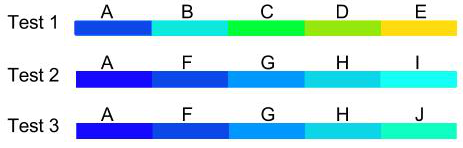
\includegraphics[width=6cm,height=3cm]{spectra.png}
\caption{A figurative spectra where each colour represents different method execution details. We see similarities between Test 2 and 3. In contrast, Test 1 is different from 2 and 3. }
\label{fig:spectra}
\end{figure}

It is important to understand the dangers of removing test cases. Unless two test cases are exactly the same, it is difficult to guarantee that they are redundant, even if one subsumes another. Therefore the aim of the project is to create a framework that gives developers different approaches in identifying redundant test cases. The framework should allow a developer to configure different analysis metrics and view the results through an output file. This means that the framework is useful for gaining an overview and understanding of the condition of the current test suite, allowing for manual inspection to determine if potentially redundant tests are actually redundant.

Another potential use case of the framework is to redistribute the test cases. This can be achieved through the splitting of any highly redundant tests into separate test suites and running the suites at different times, ensuring the original bug finding ability is retained. For example, one test suite can be run during continuous integration, and the other over night.
David Pearce is currently writing a language called Whiley, which contains an extended static checking framework in order to eliminate run time exceptions through formal verification techniques. In the compiler module alone, there are roughly 1500 tests. Relocating a number of these tests into another suite would result in allowing David Pearce to increase development speed due to a reduction in the time taken to run a large test suite. Frequent execution of tests allows for bugs to be traced back to code changes, using a smaller suite for every few changes means it will take less time to execute. The bug finding ability is not affected due to being able to run the full suite when development is not being done. 

Other papers examining this research area identify redundant tests using statement information, our research explored throughout the report will be using method coverage. The majority of the previous studies examined bench marks with under 1,000 test cases. For bench marks with over 1,000 cases storing every statement execution could be costly. Therefore it would be intriguing to see to what extent can method execution data identify redundant test cases. One of the issues that previous studies reported were high level of false positive. Method execution data gives a few different ways to explore this issue which are explored in Section \ref{S:metrics}. The aim of the paper is split into two sections: 

\begin{itemize}
\item Create a framework to identify redundant test cases
\item Analyse different strategies to identify redundant test cases through experimenting on realistic benchmarks
\end{itemize}


